\documentclass[10pt]{beamer}


\mode<presentation>
{
  \usetheme{metropolis}      % or try Darmstadt, Madrid, Warsaw, ...
  \usecolortheme{seahorse} % or try albatross, beaver, crane, ...
  \usefonttheme{default}  % or try serif, structurebold, ...
  \setbeamertemplate{navigation symbols}{}
  \setbeamertemplate{caption}[numbered]
} 

\makeatletter
\newif\if@mathitemize
\newif\if@closemathitem
\let\orig@item=\item
\renewcommand{\item}{\if@closemathitem$\fi\orig@item\if@mathitemize\@closemathitemtrue$\fi}
\newenvironment{mathitemize}{\@mathitemizetrue\itemize\@closemathitemfalse}{$\enditemize}
\makeatother

\makeatletter
\newcommand{\mtmathitem}{%
\xpatchcmd{\item}{\@inmatherr\item}{\relax\ifmmode$\fi}{}{\errmessage{Patching of \noexpand\item failed}}
\xapptocmd{\@item}{$}{}{\errmessage{appending to \noexpand\@item failed}}}
\makeatother

\newenvironment{mathitem}[1][]{%
\itemize[#1]\mtmathitem}{$\endlist}                    %$

\newenvironment{mathenum}[1][]{%
\enumerate[#1]\mtmathitem}{$\endlist}                  %$

\newenvironment{mathdesc}[1][]{%
\description[#1]\mtmathitem}{$\endlist} 

\usepackage{ragged2e}
\usepackage{etoolbox}
\usepackage{lipsum}
\usepackage[absolute,overlay]{textpos}
\usepackage{graphicx}

\apptocmd{\frame}{}{\justifying}{}

\usepackage[english]{babel}
%\usepackage[utf8x]{inputenc}
\usepackage{colortbl}
\graphicspath {{figures/}}
\usepackage[font=scriptsize,labelfont=bf]{caption}


\setbeamercolor{bibliography item}{parent=palette primary}
\setbeamertemplate{bibliography entry title}{}
\setbeamertemplate{bibliography entry location}{}
\setbeamertemplate{bibliography entry note}{}
\setbeamertemplate{bibliography item}{\insertbiblabel}


%% GRID %%
\usepackage{tikz}
\usetikzlibrary{arrows,decorations.markings}
\usetikzlibrary{decorations.pathreplacing}

\newcommand{\grid}{
 \begin{tikzpicture}[overlay,remember picture]
   \begin{scope}[shift={(current page.south west)}]
     \draw[gray!50] (0,0) grid[step=2mm] (current page.north east);
     \draw[red!50] (0,0) grid[step=1cm] (current page.north east);
     \draw (0.2,1) node {1};
     \draw (0.2,2) node {2};
     \draw (0.2,3) node {3};
     \draw (0.2,4) node {4};
     \draw (0.2,5) node {5};
     \draw (0.2,6) node {6};
     \draw (0.2,7) node {7};
     \draw (0.2,8) node {8};
     \draw (0.2,9) node {9};
     \draw (1,0.5) node {1};
     \draw (2,0.5) node {2};
     \draw (3,0.5) node {3};
     \draw (4,0.5) node {4};
     \draw (5,0.5) node {5};
     \draw (6,0.5) node {6};
     \draw (7,0.5) node {7};
     \draw (8,0.5) node {8};
     \draw (9,0.5) node {9};
     \draw (10,0.5) node {10};
     \draw (11,0.5) node {11};
     \draw (12,0.5) node {12};
   \end{scope}
 \end{tikzpicture}
 }
 
%%

\title{DAIT Project}
\subtitle{Trajectory Preduiction for Human-Human Interaction}
\author{Rodolphe Farrando, Romain Gratier}%\\[1cm] {\small Supervisors: Nicholas Molyneaux, Ga�l Lederrey, Michel Bierlaire}}
\institute{EPFL}
\date{23.05.2018}


\begin{document}

\begin{frame}[noframenumbering]
  \maketitle
  \thispagestyle{empty}
\end{frame}

\begin{frame}[noframenumbering]{Table of contents}
\thispagestyle{empty}
  \setbeamertemplate{section in toc}[sections numbered]
  \vspace{0.6cm}
  \tableofcontents[hideallsubsections]
\end{frame}

%%%%%%%%%%%%%%%%%%%%%%% INTRODUCTION %%%%%%%%%%%%%%%%%%%%%%% 

\section{Introduction}
\begin{frame}{Introduction}
Motivation:
\begin{itemize}
\onslide<1->{\item Trajectory prediction is crucial for improving autonomous vehicles behaviour}
\onslide<2->{\item Could avoid situations seen in the ethical lectures}
\end{itemize}

\begin{center}
\begin{overprint}
\onslide<1> \centerline {\includegraphics[scale = 0.3]{figure/intro1}}
\onslide<2->\centerline {\includegraphics[scale = 0.3]{figure/intro2}}
\end{overprint}
\end{center}


%Goal:
%\begin{itemize}
%\item Find model which predict trajectories better than linear prediction
%\item Predict coordinates
%\end{itemize}
\end{frame}
%%%%%%%%%%%%%%%%%%%%%%% LITERATURE %%%%%%%%%%%%%%%%%%%%%%% 

\begin{frame}{Previous work Social LSTM : Human Trajectory Prediction in Crowded Spaces}
%\begin{block}{Social LSTM : Human Trajectory Prediction in Crowded Spaces}
%\end{block}


In their project, they used different components to make the structure :
\begin{itemize}
\item One LSTM per pedestrian
\item A Social Pooling
\item per frame
\end{itemize}

In our project we only use :

\begin{itemize}
\item One CNN, or one LSTM
\item per pedestrian
\end{itemize}
%The parameters of both models are standard.
\end{frame}

\section{Preprocessing and Postprocessing}
\begin{frame}{Preprocessing}
We have :\\
\begin{itemize}
\item files with pedestrians id
\item  frame number 
\item coordinates
\end{itemize}

We want :\\
\begin{itemize}
\item future coordinates
\end{itemize}

Each trajectories are divided in two (two sets of 10 x and y coordinates): 
\begin{itemize}
\item Training coordinates
\item Ground truth
\item We want to predict a sequence of 10 x and y coordinates such that they are close to the ground truth
\end{itemize}
\end{frame}


\begin{frame}{Preprocessing}
The preprocessing is divided in 4 steps:
\begin{enumerate}
\justifying
\item We isolate each trajectory along with his interaction, that is the other trajectories that are around within the same frames
\item We normalize the trajectories such that the first point is at $(0,0)$ and the second is at $(0,y_1)$
\item We calculate axis velocities $V_x$ and $V_y$
\item For each frame, if there is a interacting pedestrian we add its coordinates and speed otherwise zeros are added
\end{enumerate}
Finally our inputs have the following shape: $[10,N,4 * N_{inter}]$, with 
\begin{itemize}
\justifying
\item 10: sequence length
\item $N$: The number of data
\item $4*N_{inter}$: 4 (being the $x$ and $y$ coordinates and $V_x$ and $V_y$ velocities) times the number of pedestrians interacting with the one of interest.
\end{itemize}
\end{frame}


\begin{frame}
\frametitle{Outputs structure}
\begin{itemize}
\item The models can predict either coordinate or speed or both
\item We test our two models for 4 different cases
\end{itemize}
The four different cases are:
\begin{enumerate}
\justifying
\item Predict coordinates with loss defines as $L_1 = (X-X_{pred})^2$ with $X = [x,y]$
\item Predict speeds with loss defines as $L_2 = (V-V_{pred})^2$ with $V = [V_x,V_y]$ 
\item Predict both coordinates and speeds with loss defines as $L = L_1 + L_2$
\item Predict both coordinates and speeds with loss defines as $L = L_1 + L_2 + L_3 $, with $L_3 = (X- X_{t-1} + V_t*0.4)^2$
\end{enumerate}
The fourth case ensure that coordinates and speeds are not predicted independently.
\end{frame}




\section{Models}
\begin{frame}{CNN}
Define CNN
\end{frame}

\begin{frame}{LSTM}
\begin{figure}
\includegraphics[scale = 0.25]{figure/manytomany}
\end{figure}
\textbf{Inputs:} sequence of coordinates and velocities of the trajectory of interest and of the interacting trajectories\\
\textbf{Outputs:} sequence of predicted coordinates and velocities for the trajectory of interest 
\end{frame}

\section{Results}
\begin{frame}
\frametitle{Results: Introduction}
To calculate the correctness of the prediction two indicators are used:
\begin{enumerate}
\item The final displacement error: $e_{fin} = \sqrt{(X_{n}-X_{pred,n})^2}$
\item The mean displacement error: $e_{fin} = \sqrt{\frac{\sum_{i=0}^n(X_{gt,i}-X_{pred,i})^2}{(n)}}$
\end{enumerate}
Depending on the inputs two ways are possible to find the predicted coordinates:
\begin{enumerate}
\item If the coordinates are predicted: directly use them
\item If the velocities are predicted: $X_{t} = X_{t-1} + V_{t}\cdot 0.4$, with $0.4$ the time between two frames in seconds
\end{enumerate}
\end{frame}

\begin{frame}
\frametitle{Results: LSTM}
\begin{table}[]
\centering
\begin{tabular}{c|c|c|c|c|c|c|}
\cline{2-7}
                                     & \multicolumn{3}{c|}{Model 3}   & \multicolumn{3}{c|}{Model 4}   \\ \cline{2-7} 
                                     & \multicolumn{3}{c|}{Traj type} & \multicolumn{3}{c|}{Traj type} \\ \cline{2-7} 
                                     & 1         & 2        & 3       & 1         & 2        & 3       \\ \hline
\multicolumn{1}{|c|}{Mean disp. L2}  & 0.519     & 0.484    & 0.568   & 0.537     & 0.473    & 0.576   \\ \hline
\multicolumn{1}{|c|}{Final disp. L2} & 0.979     & 0.871    & 1.093   & 0.992     & 0.86     & 1.125   \\ \hline
\end{tabular}
\end{table}
\end{frame}


\section{Representation}








\end{document}